\documentclass[aspectratio=169]{beamer}
\usepackage{color,amsmath}
\usepackage{subfigure}
\usepackage{booktabs}
\usepackage{framed}
\usepackage{comment}

\usepackage{hyperref}
\hypersetup{
    colorlinks=true,
    linkcolor=blue,
    filecolor=magenta,      
    urlcolor=cyan,
}

%%%%%%%%%%%%%%%%%%%%%%%%%%
\title[]{\textcolor{gray}{[What, why, and which experiments?], \newline [Moving beyond simple experiments], [Making it happen]},\newline [Zero variable cost data and MusicLab],  \textcolor{gray}{[3 Rs]}}
\author[]{Matthew J. Salganik\\Department of Sociology\\Princeton University}
\date[]{
\begin{flushright}

\includegraphics[width=0.1\textwidth]{figures/cc-by.png}
\end{flushright}
}
\begin{document}
%%%%%%%%%%%%%%%%%%%%%%%%%%
\frame{\titlepage}
%%%%%%%%%%%%%%%%%%%%%%%%%%
\begin{frame}

\begin{columns}
\begin{column}{.40\textwidth}
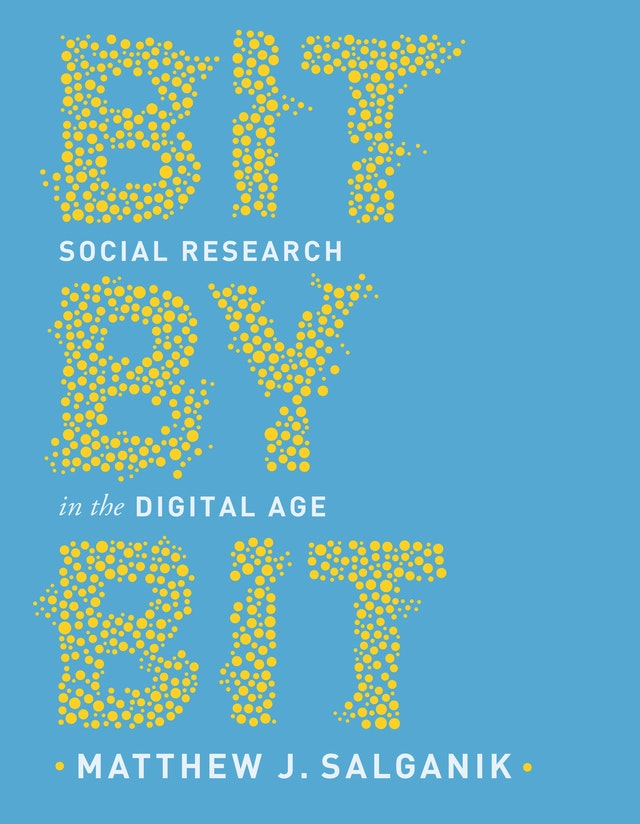
\includegraphics[width=\textwidth]{figures/salganik_bit_2018_cover}
\end{column}%

\hfill%

\begin{column}{.60\textwidth}
1) Introduction \\
2) Observing behavior \\
3) Asking questions \\
\textcolor{blue}{4) Running experiments} \\
5) Mass collaboration \\
6) Ethics \\
7) The future \\
\end{column}%
\end{columns}

\end{frame}
%%%%%%%%%%%%%%%%%%%%%%
\begin{frame}

{\Large
\begin{center}
Experiments at scale
\end{center}
}
\end{frame}
%%%%%%%%%%%%%%%%%%%%%%%%%
\begin{frame}

\begin{center}
\only<1>{\includegraphics[width=0.8\textwidth]{figures/zero_variable_cost_experiments_analog}}
\only<2>{\includegraphics[width=0.8\textwidth]{figures/zero_variable_cost_experiments_both}}
\end{center}

\end{frame}
%%%%%%%%%%%%%%%%%%%%%%%%%
\begin{frame}

Main sources of variable costs:
\begin{itemize}
\item staff time
\item participant payment
\end{itemize}

\vfill
\pause
Solutions:
\begin{itemize}
\item Automation (your experiments should run while you sleep)
\item Design enjoyable experiments
\end{itemize}

\end{frame}
%%%%%%%%%%%%%%%%%%%%%%%%
\begin{frame}

\begin{figure}
  \centering
  \includegraphics[width = 0.9\textwidth]{figures/splashscreen}
\end{figure}

\end{frame}
%%%%%%%%%%%%%%%%%%%%%%%%%%%%%%%%%
\begin{frame}

\begin{figure}
  \centering
  \includegraphics[width = 0.9\textwidth]{figures/info-v1-cut}
\end{figure}

\end{frame}
%%%%%%%%%%%%%%%%%%%%%%%%%%%%%%%%%
\begin{frame} 

\begin{figure}
  \centering
  \includegraphics[width = 0.9\textwidth]{figures/listenscreen}
\end{figure}

\end{frame}
%%%%%%%%%%%%%%%%%%%%%%%%%%%%%%%%%
\begin{frame}

\begin{figure}
  \centering
  \includegraphics[width = 0.9\textwidth]{figures/downloadscreen}
\end{figure}

\end{frame}
%%%%%%%%%%%%%%%%%%%%%%%%%%%%%%%%%%
\begin{frame}

\begin{figure}
  \centering
  \includegraphics[width = 0.9\textwidth]{figures/info-v1-cut}
\end{figure}

\end{frame}
%%%%%%%%%%%%%%%%%%%%%%%%%%%%%%%%%
\begin{frame}

  \begin{columns}
    \column{0.4\textwidth}
     \begin{block}{}
       
\includegraphics[width=\textwidth]{figures/hp-cover.pdf}
     \end{block}

   \pause
   
   \column{0.6\textwidth}
     \begin{block}{}
       \begin{itemize}
         \item Wild success \pause
         \item Rejected by eight publishers\\
       \end{itemize}
     \end{block}
  \end{columns}

\end{frame}
%%%%%%%%%%%%%%%%%%%%%%%%
\begin{frame}

  \begin{columns}
    \column{0.4\textwidth}
     \begin{block}{}
       
\includegraphics[width=\textwidth]{figures/star-wars}
     \end{block}
   
   \column{0.6\textwidth}
     \begin{block}{}
       \begin{itemize}
         \item Set box office records, won 6 Oscars, and launched a multi-billion dollar franchise
         \item Rejected by United Artists and Universal before being made by Fox
       \end{itemize}
     \end{block}
  \end{columns}

\end{frame}
%%%%%%%%%%%%
\begin{frame}

  \begin{columns}
    \column{0.4\textwidth}
     \begin{block}{}
       
\includegraphics[width=\textwidth]{figures/american-idol}
     \end{block}

   \column{0.6\textwidth}
     \begin{block}{}
       \begin{itemize}
         \item One of the most popular shows of the decade
         \item Rejected by ABC, CBS, and NBC before being picked up by Fox
       \end{itemize}
     \end{block}
  \end{columns}

\end{frame}
%%%%%%%%%%%%%%%%
\begin{frame}

Puzzling nature of success for cultural objects (books, movies, piece of art, music, TV shows)
\begin{itemize}
  \item<1-> {extreme inequality in success}
  \item <2->{unpredictability of success}
\end{itemize}

\end{frame}
%%%%%%%%%%%%%%%%%%%%%%%%%%%%%%%
\begin{frame} 

\begin{figure}
  
\includegraphics[width = 0.8\textwidth]{figures/musiclab_model}
\end{figure}

\end{frame}
%%%%%%%%%%%%%%%%%%%%%%%%%%%%%%%%%%
\begin{frame}

\begin{figure}
  \centering
  \includegraphics[width=0.9\textwidth]{figures/expdesign_4}
\end{figure}

\end{frame}
%%%%%%%%%%%%%%%%%%%%%%%%%%%%%%%%%%
\begin{frame}

\setcounter{subfigure}{0}
\begin{figure}
  \centering
     \subfigure[Less social influence]{
     \includegraphics[width=0.45\textwidth]{figures/info-v1-cut}}
  \hspace{0in}
     \subfigure[More social influence]{
     \includegraphics[width=0.45\textwidth]{figures/info-v2-original}}
\end{figure}

\end{frame}
%%%%%%%%%%%%%%%%%%%%%%%%%%%%%%%%%%
\begin{frame}

\begin{figure}
  \centering
  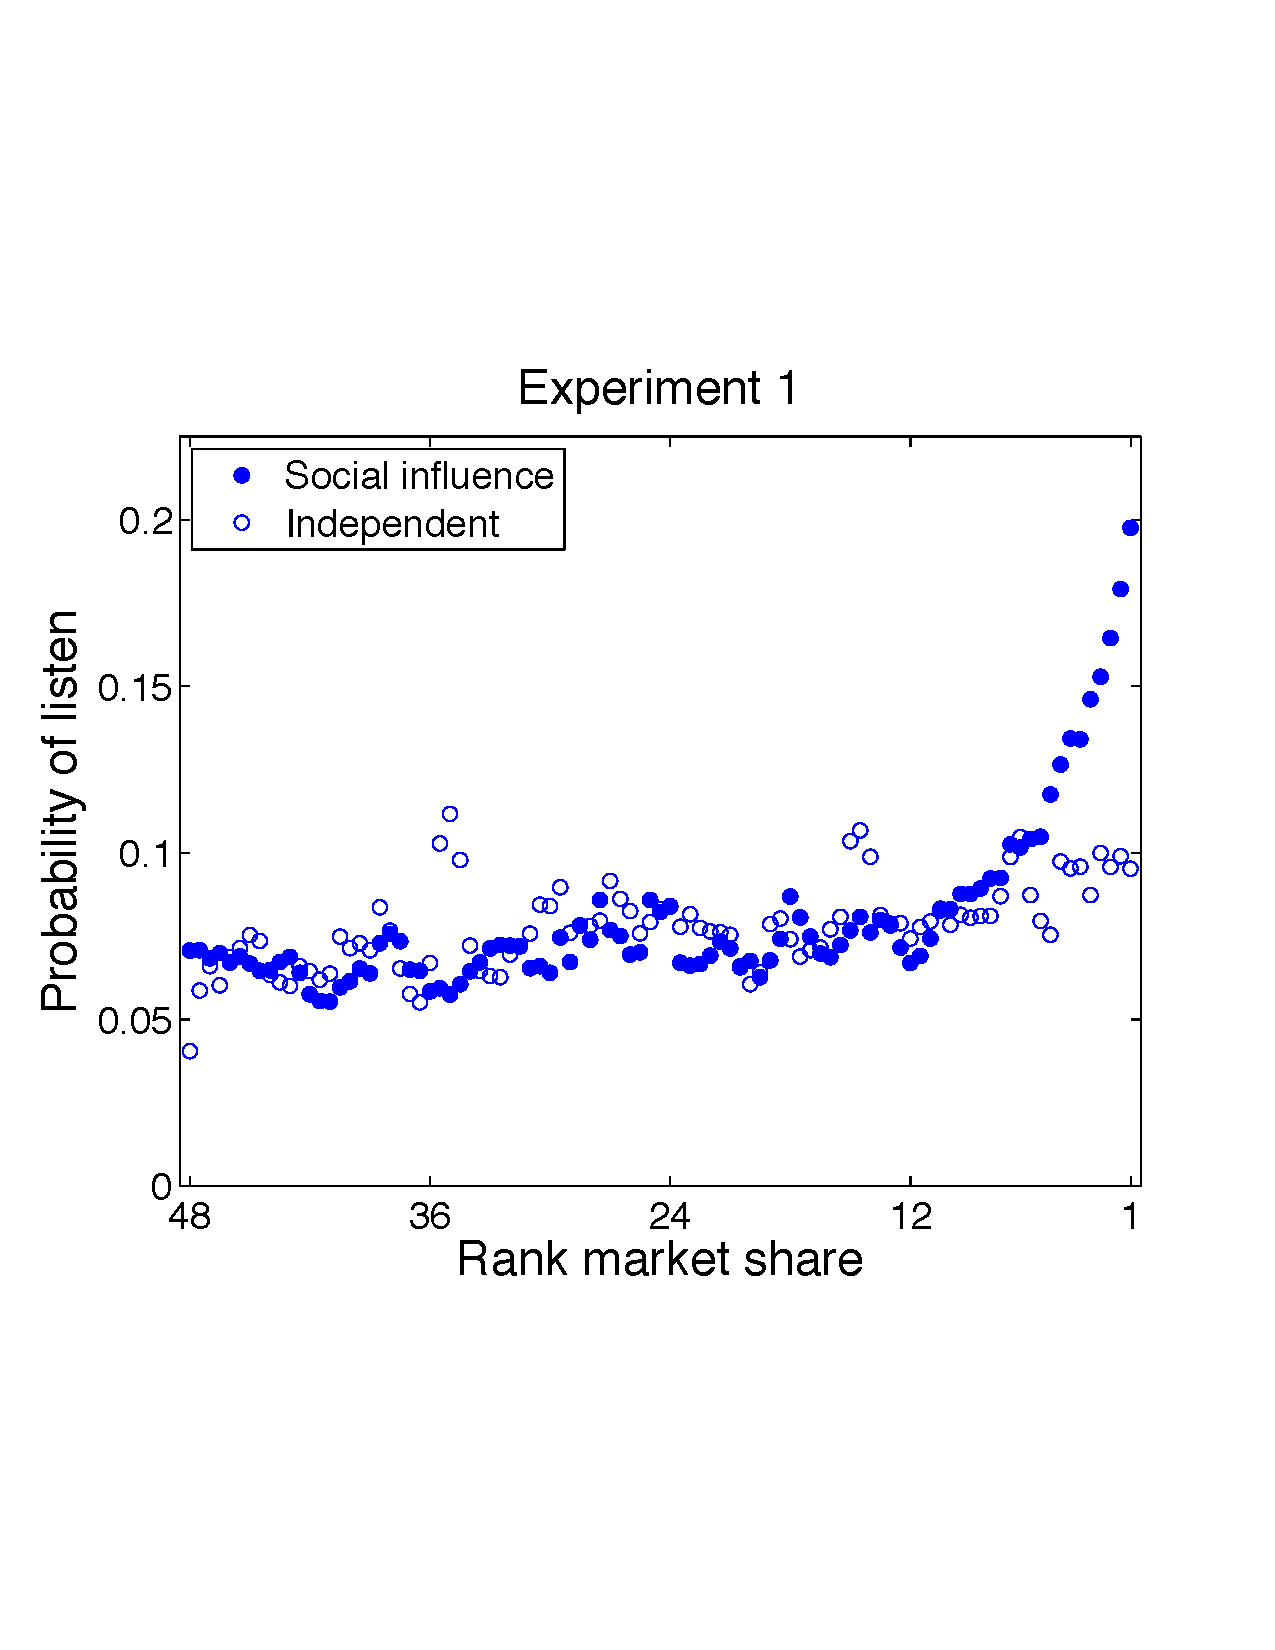
\includegraphics[width= 0.6\textwidth]{figures/listenchoice_v1_smoothed_1}
\end{figure}

\end{frame}
%%%%%%%%%%%%%%%%%%%%%%%%%%%%%%%%%%%%%%%%%%%
\begin{frame}

\setcounter{subfigure}{0}
\begin{figure}
  \centering
     \subfigure[Experiment 1, weaker signal]{
     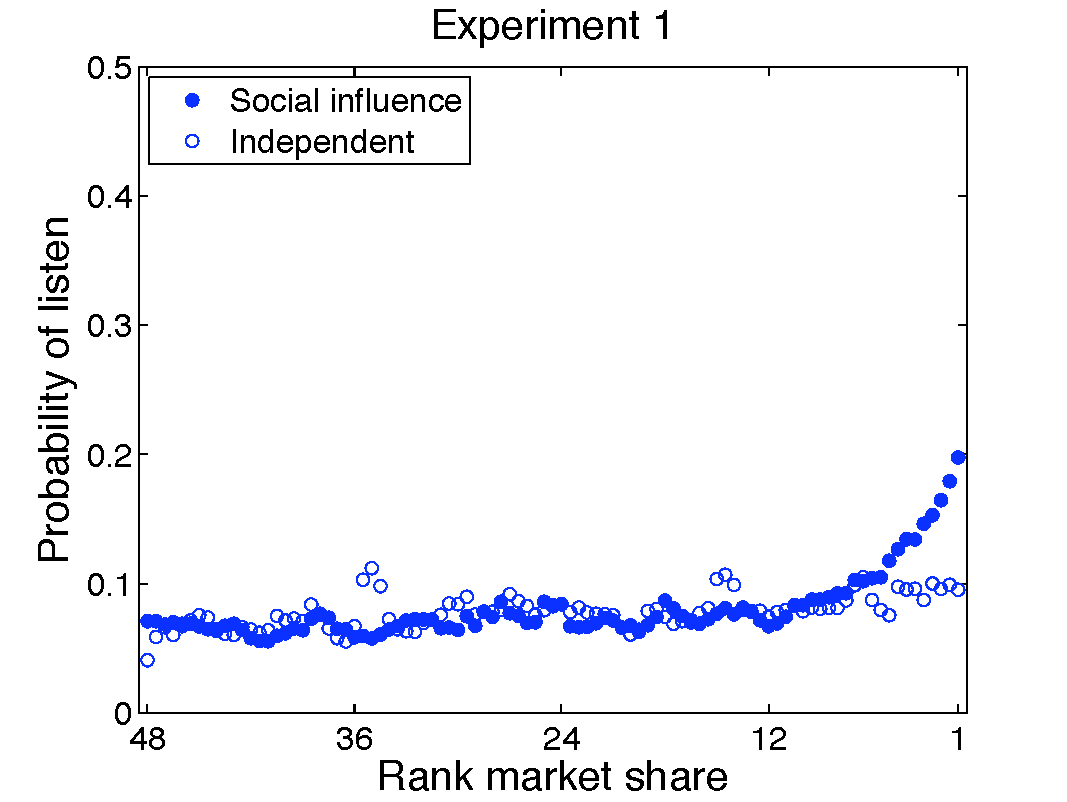
\includegraphics[width=0.45\textwidth]{figures/listenchoice_v1_v2scale_smoothed_1}}
  \hspace{0in}
    \subfigure[Experiment 2, stronger signal]{
     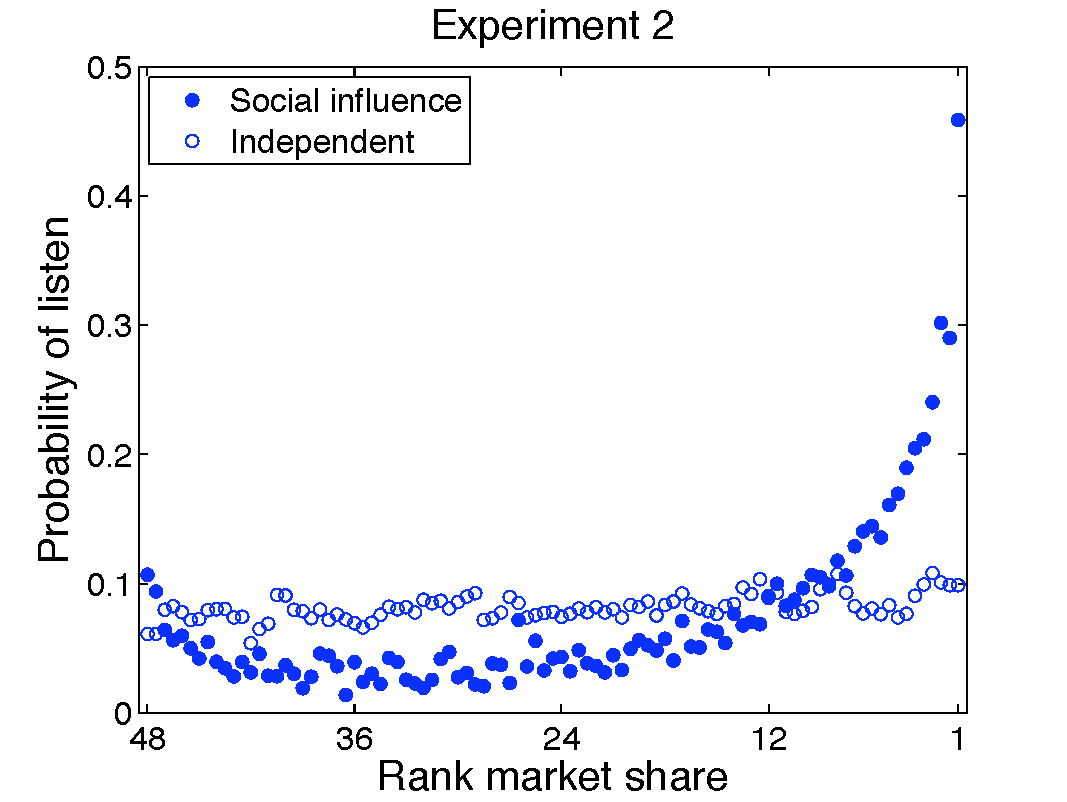
\includegraphics[width=0.45\textwidth]{figures/listenchoice_v2_smoothed}}
\end{figure}

\end{frame}

%%%%%%%%%%%%%%%%%%%%%%%%%%%%%%%%%%
\begin{frame}

\begin{figure}
  \centering
  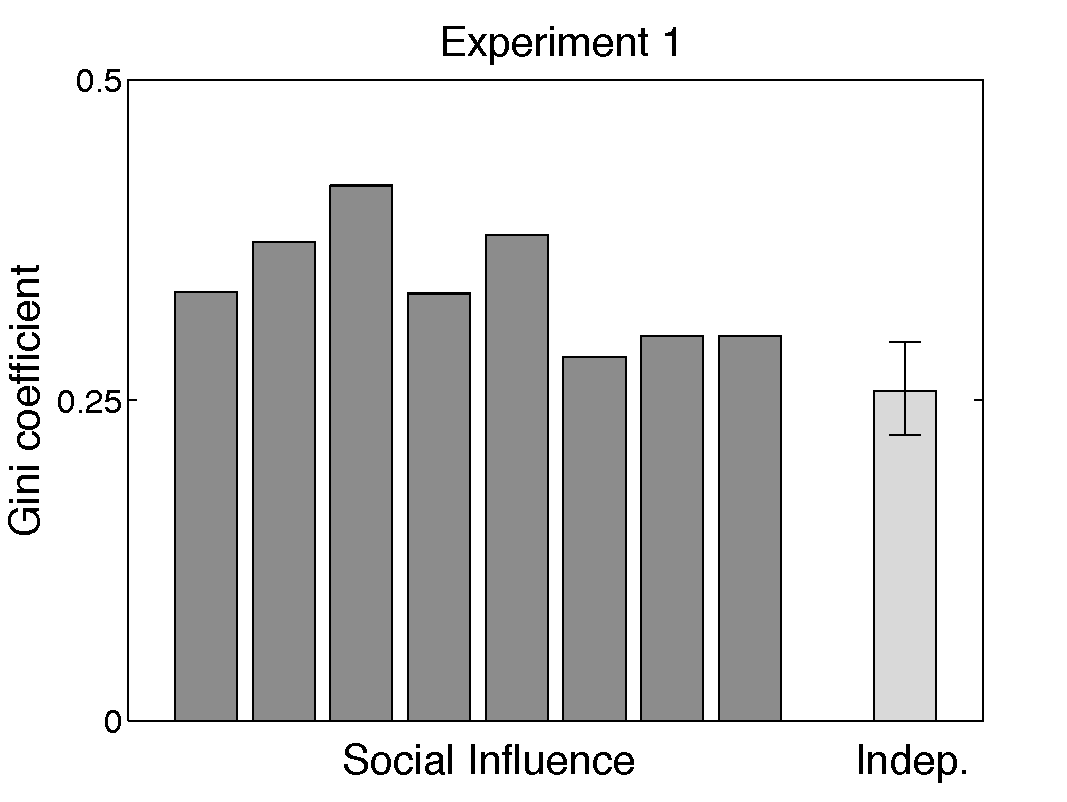
\includegraphics[width=0.7\textwidth]{figures/gini_v1_unordered_ci}
\end{figure}

\end{frame}
%%%%%%%%%%%%%%%%%%%%%%%%%%%%%%%%%%%%%%%%%%%%
\begin{frame}

\begin{figure}
  \centering
  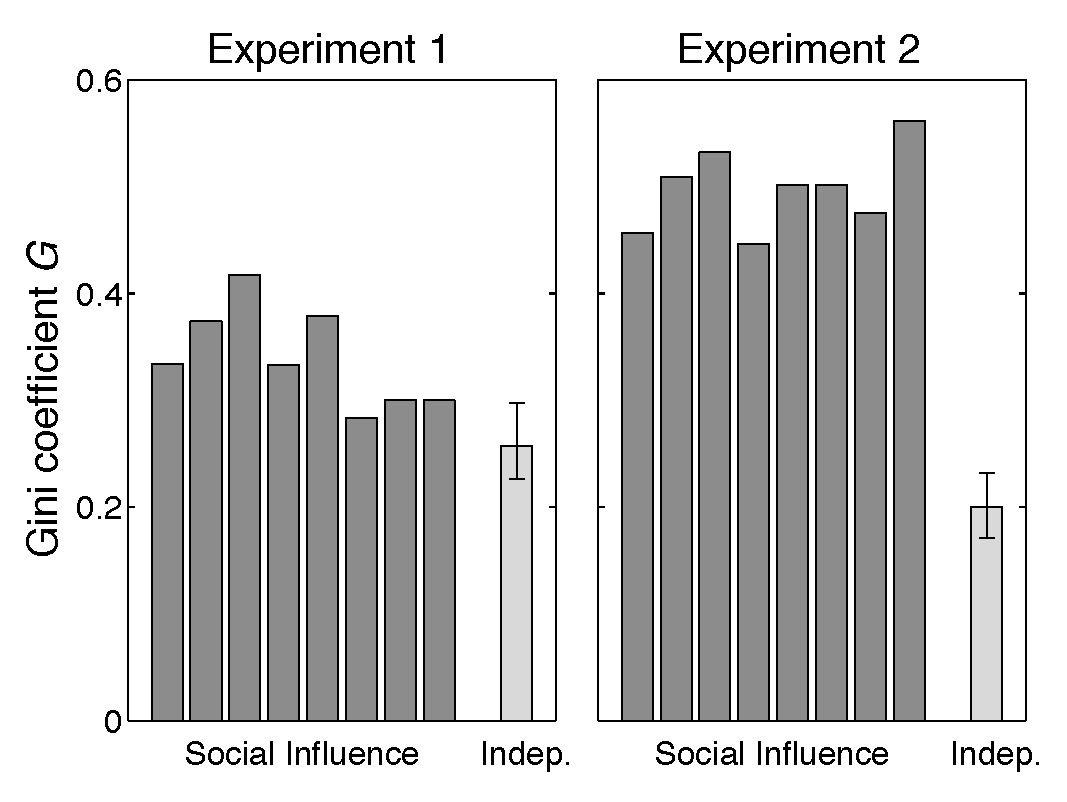
\includegraphics[width=3in]{figures/compare_gini_v1v2_unordered_ci}
\end{figure}

Median Gini coefficient increases from $0.34$ (France) to $0.50$ (Nigeria)
\end{frame}

%%%%%%%%%%%%%%%%%%%%%%%%%%%%%%%%%
\begin{frame}

$U$ = mean difference in market share across all pairs of realizations\\
\begin{figure}
  \centering
  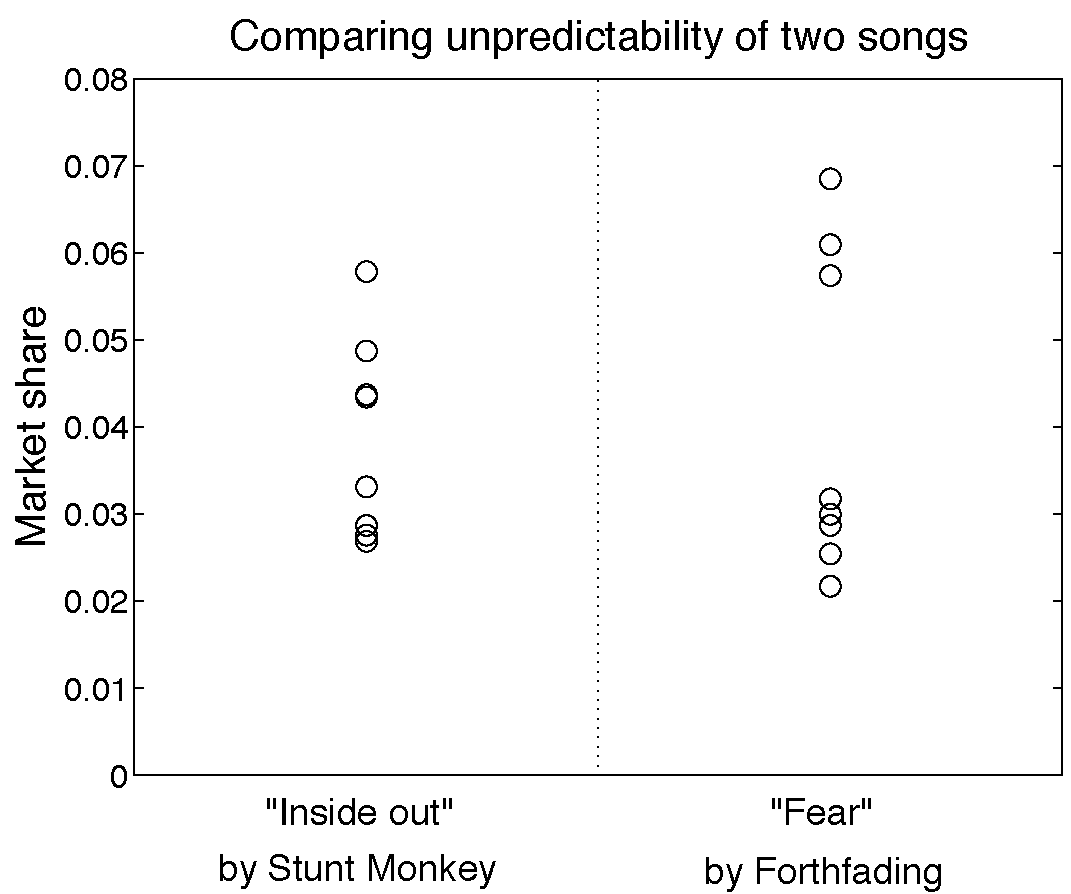
\includegraphics[width = 3in]{figures/arbitrary_example}
\end{figure}

\end{frame}
%%%%%%%%%%%%%%%%%%%%%%%%%%
\begin{frame}

\begin{figure}
  \centering
  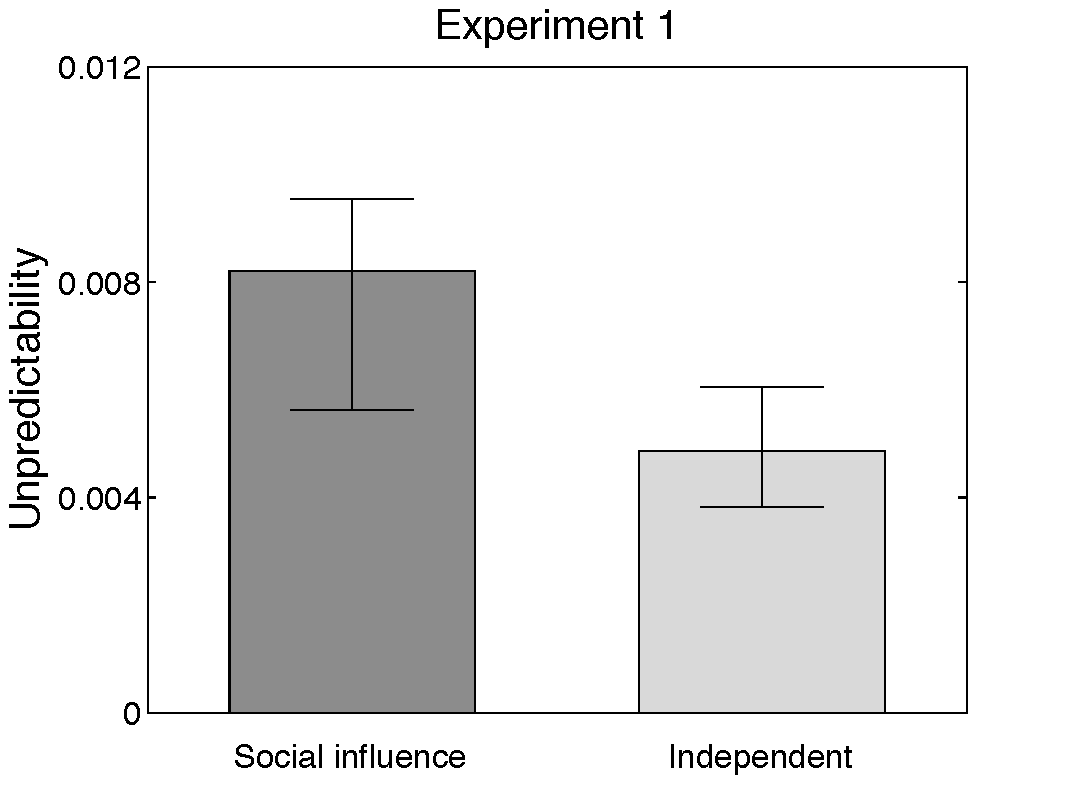
\includegraphics[width = 3.5in]{figures/unpredictability_v1}
\end{figure}

\end{frame}
%%%%%%%%%%%%%%%%%%%%%%%%%%%%
\begin{frame}

\begin{figure}
  \centering
  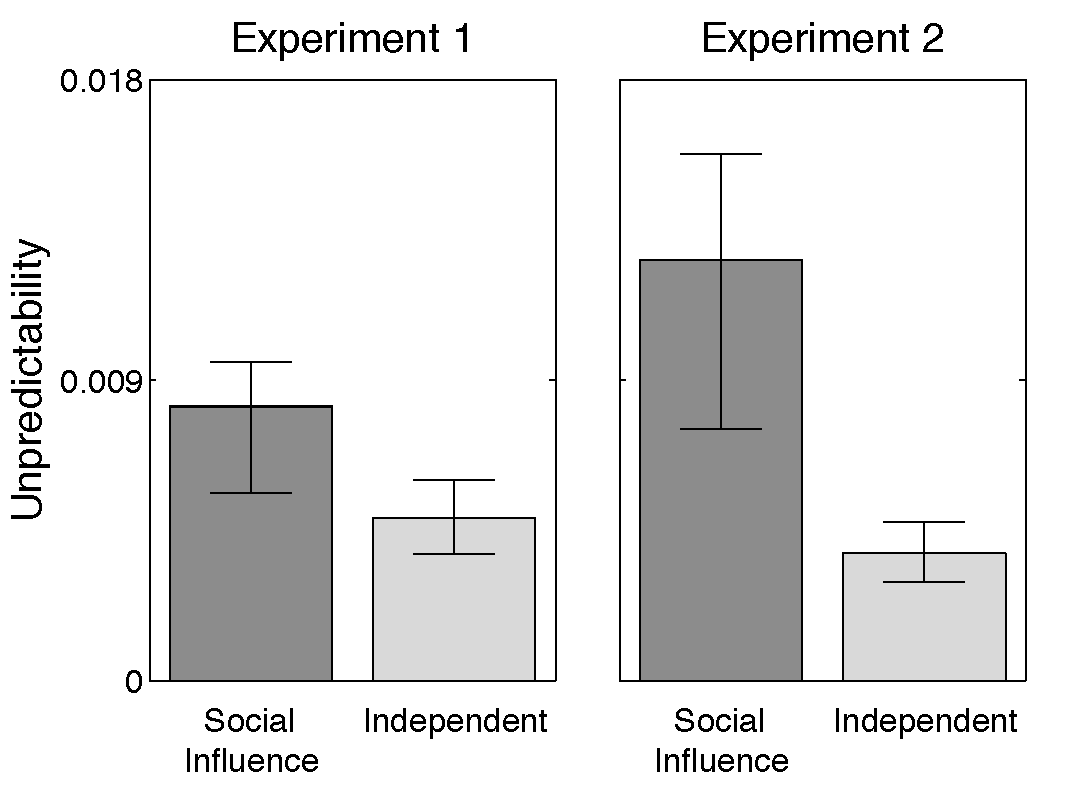
\includegraphics[width=3in]{figures/compare_unpred_v1v2}
\end{figure}

Unpredictability increases by about 50\%
\end{frame}
%%%%%%%%%%%%%%%%%%%%%%%%%%%%%%%%%
\begin{frame}

Experiments 1 and 2 show a dose-response relationship.  Increasing the strength of social influence leads to

\begin{itemize}
  \item increased inequality of success
  \item increased unpredictability of success
\end{itemize}

\end{frame}
%%%%%%%%%%%%%%%%%%%%%%%%%%%%%%%%%
\begin{frame}

What is the relationship between ``quality'' and success?

\end{frame}
%%%%%%%%%%%%%%%%%%%%%%%%%%%%%%%%
\begin{frame}

\begin{figure}
  \centering
  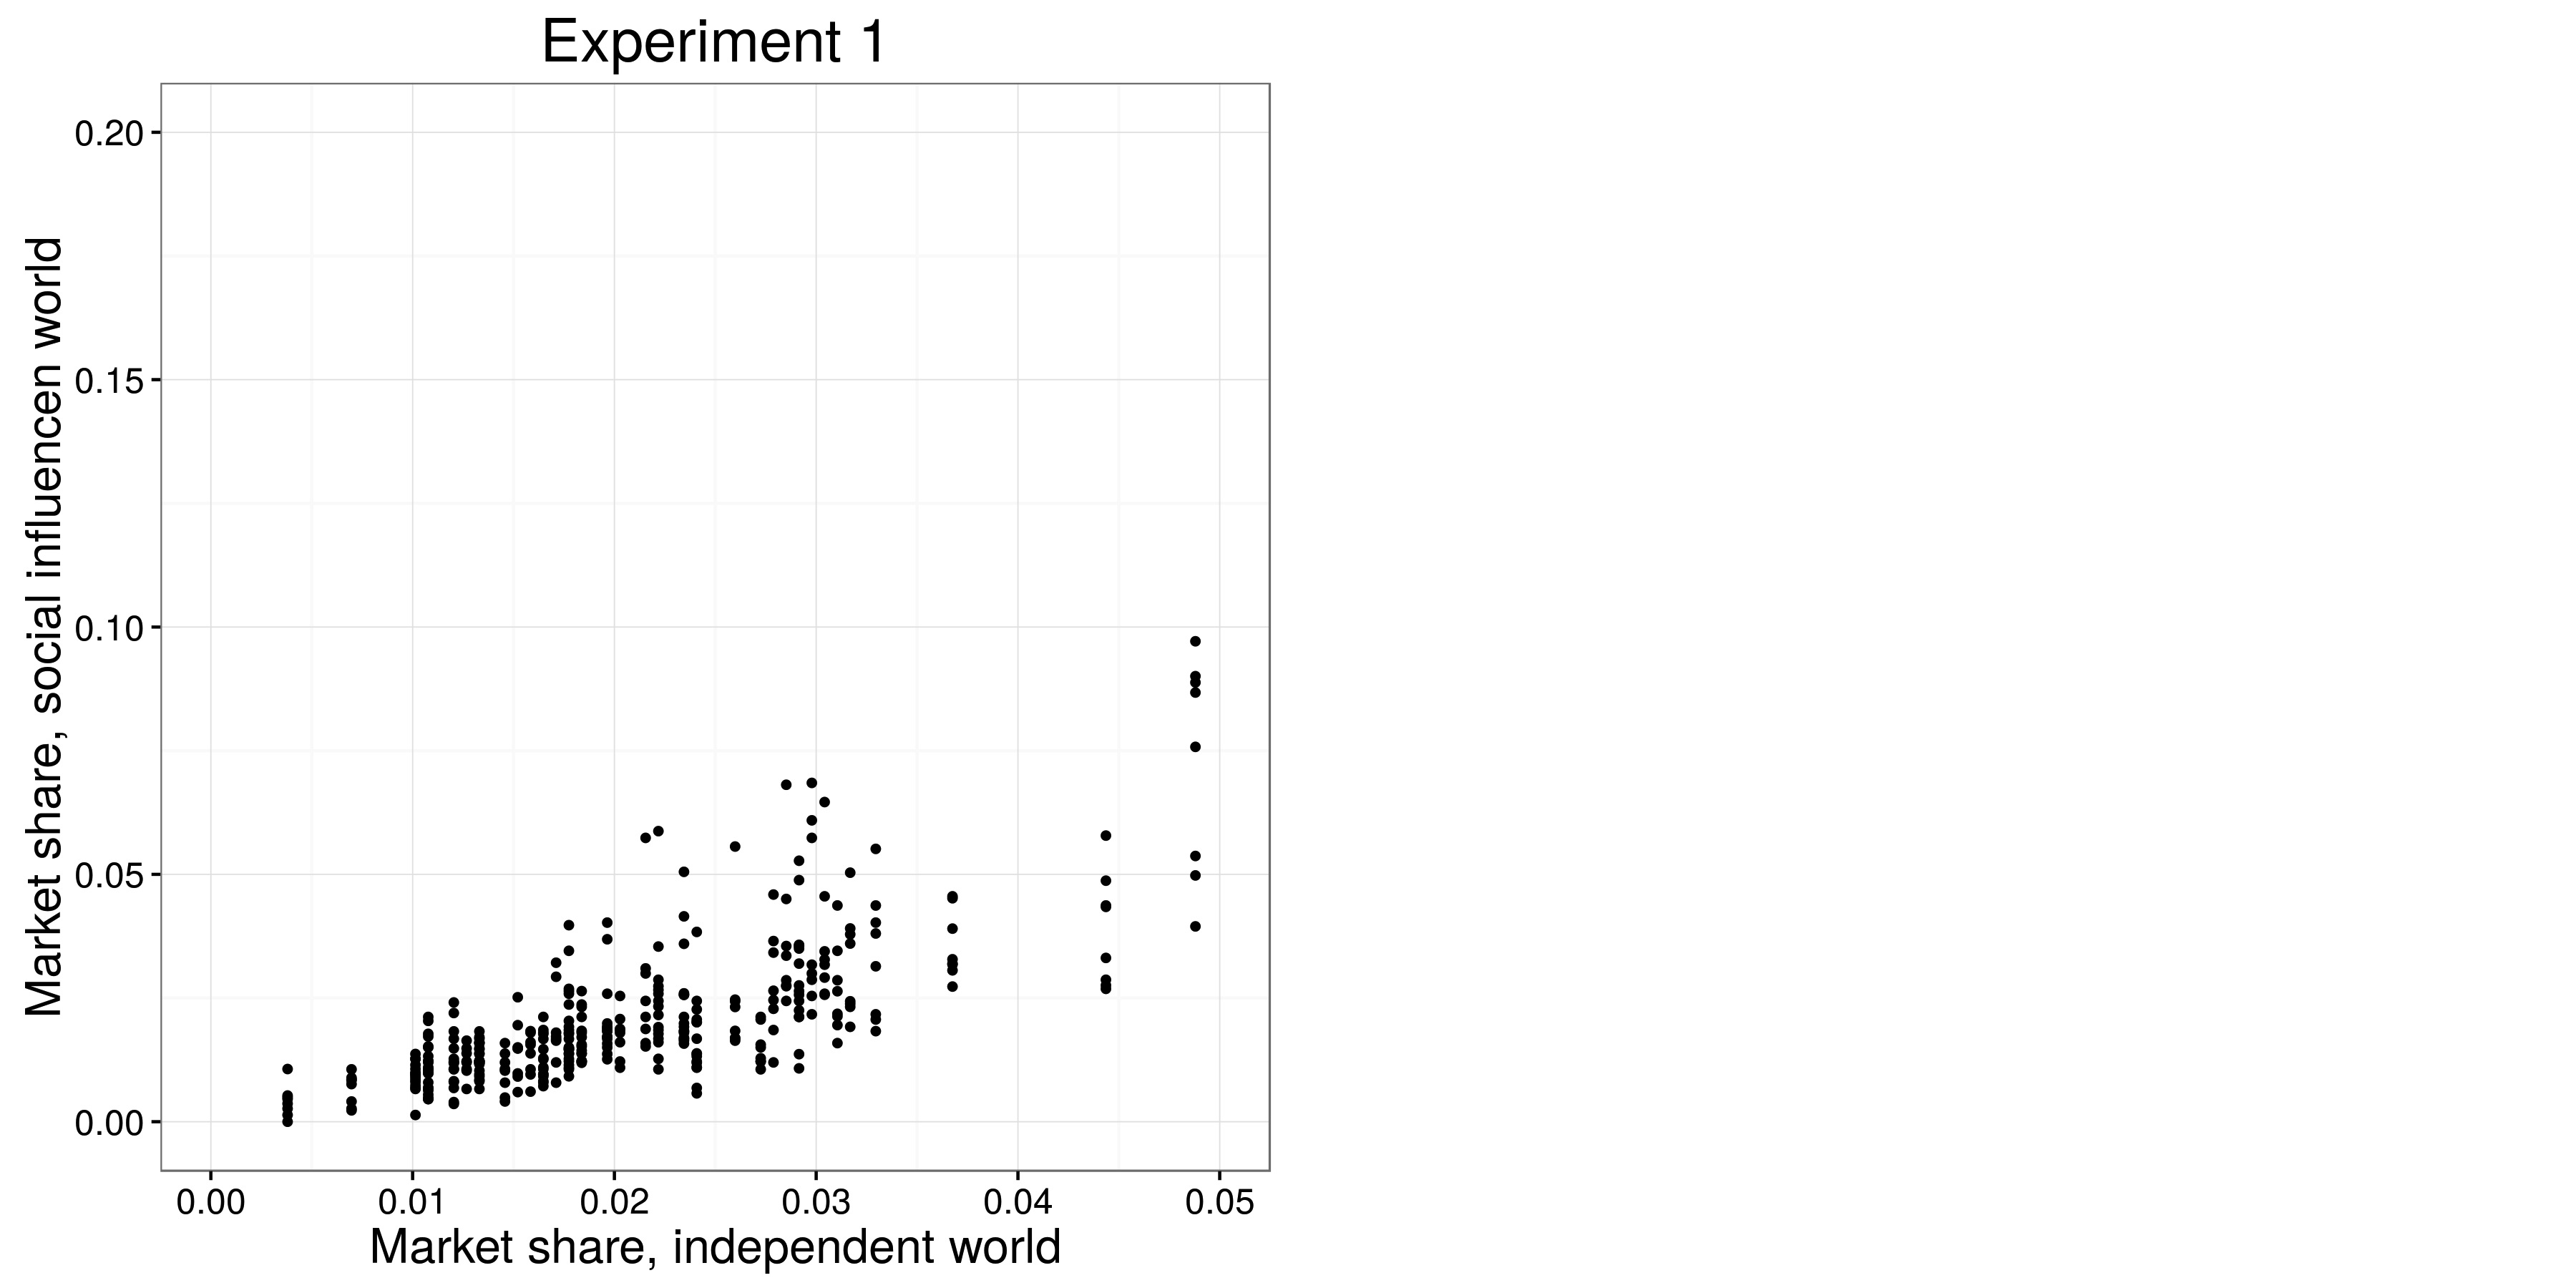
\includegraphics[width=0.85\textwidth]{figures/bitbybit4-23_salganik_experimental_2006_fig3a}
\end{figure}

\end{frame}
%%%%%%%%%%%%%%%%%%%%%%%%%%%%%%%%%%
\begin{frame}

\begin{figure}
  \includegraphics[width=0.85\textwidth]{figures/bitbybit4-23_salganik_experimental_2006_fig3ac}
\end{figure}

Results: \pause
\begin{itemize}
\item More social influence leads to more unpredictability
\pause
\item You can predict failure but you can't predict success
\pause 
\item \href{http://dx.doi.org/10.1126/science.1121066}{Salganik, Dodds, and Watts (2006)}
\end{itemize}
 
\end{frame}
%%%%%%%%%%%%%%%%%%%%%%%%%%%%%%%%%%
\begin{frame}

\begin{figure}
  \centering
  \includegraphics[width=0.7\textwidth]{figures/zero_variable_cost_experiments_musiclab}
\end{figure}

\vfill
\pause
\Large{Zero variable cost is a means not an end.}

\end{frame}
%%%%%%%%%%%%%%%%%%%%%%%%
\begin{frame}

\begin{figure}
  \centering
  \includegraphics[width=0.8\textwidth]{figures/milkman_temporal_2012_title.png}
\end{figure}

\vfill
\tiny{\url{http://dx.doi.org/10.1177/0956797611434539}}

\end{frame}
%%%%%%%%%%%%%%%%%%%%%%%%
\begin{frame}

{\texttt
Dear Professor Salganik,\\ 

I am writing you because I am a prospective Ph.D. student with considerable interest in your research. My plan is to apply to Ph.D. programs this coming fall, and I am eager to learn as much as I can about research opportunities in the meantime.\\

I will be on campus today, and although I know it is short notice, I was wondering if you might have 10 minutes when you would be willing to meet with me to briefly talk about your work and any possible opportunities for me to get involved in your research. Any time that would be convenient for you would be fine with me, as meeting with you is my first priority during this campus visit.\\

Thank you in advance for your consideration.\\

Sincerely,\\
Carlos Lopez
}

\end{frame}
%%%%%%%%%%%%%%%%%%%%%%%%
\begin{frame}

\begin{figure}
  \centering
  \includegraphics[height=0.8\textheight]{figures/milkman_temporal_2012_fig1.png}
\end{figure}

\end{frame}
%%%%%%%%%%%%%%%%%%%%%%%%
\begin{frame}

\begin{figure}
  \centering
  \includegraphics[width=0.8\textwidth]{figures/milkman_temporal_2012_fig2b.png}
\end{figure}

\end{frame}
%%%%%%%%%%%%%%%%%%%%%%%%
\begin{frame}

What are the fixed and variable costs for this experiment?

\end{frame}
%%%%%%%%%%%%%%%%%%%%%%%%
\begin{frame}

{\Large
\begin{center}
Important difference between:\\
zero variable cost and zero variable cost to you
\end{center}
}

\end{frame}
%%%%%%%%%%%%%%%%%%%%%%%%
\frame{\titlepage}
%%%%%%%%%%%%%%%%%%%%%%%%%%


\end{document}
